\section*{Problem Statement}
The objective of this problem is to interpolate a polynomial for the energy levels of the hydrogen atom given discrete data points for the first five principal quantum numbers ($n=1,2,3,4,5$). The aim is to approximate the continuous energy function and visualize its variation with respect to $n$.

\begin{quote}
  \textbf{NOTE}: The code can be accessed using this link: \href{https://raw.githubusercontent.com/HavokSahil/computational-techniques-assignments/refs/heads/main/assignment4/a2.m}{MATLAB}, \href{https://raw.githubusercontent.com/HavokSahil/computational-techniques-assignments/refs/heads/main/assignment4/a2.jl}{Julia}.
\end{quote}


\section*{Background}
According to the Bohr model of the hydrogen atom, the energy levels are given by:
\[
E_n = -\frac{13.6}{n^2} \quad \text{(in eV)}.
\]
For $n=1,2,3,4,5$, this yields the values:
\[
E = \{-13.6, -3.40, -1.51, -0.85, -0.54\}.
\]
Instead of using the analytical expression, we construct an interpolating polynomial that passes through these data points using Newton’s Divided Difference method.

\section*{Methodology}
\subsection*{Newton’s Divided Difference Interpolation}
1. Construct a divided difference table $D$ with:
\[
D[i,1] = E_i, \quad D[i,j] = \frac{D[i,j-1] - D[i-1,j-1]}{n_i - n_{i-j+1}}, \quad j \geq 2.
\]
2. Form the interpolating polynomial:
\[
P(x) = \sum_{k=1}^N \left( D[k,k] \prod_{j=1}^{k-1}(x - n_j) \right).
\]
3. Evaluate $P(x)$ over a fine grid of $n$ values to approximate the energy function.

\subsection*{Steps}
\begin{enumerate}
  \item Take discrete quantum numbers $T = \{1,2,3,4,5\}$ and corresponding energies $E = \{-13.6, -3.40, -1.51, -0.85, -0.54\}$.
  \item Construct Newton’s divided difference table.
  \item Generate the interpolated polynomial curve.
  \item Plot the interpolated polynomial together with the original discrete points.
\end{enumerate}

\section*{Results}
\begin{itemize}
  \item The interpolated polynomial passed through all the given data points exactly.
  \item The polynomial curve smoothly captured the expected decreasing trend of $E_n$ with increasing $n$.
  \item The resulting interpolation matched the known theoretical expression $E_n = -13.6/n^2$ for the provided range.
\end{itemize}

\begin{figure}[h!]
  \centering
  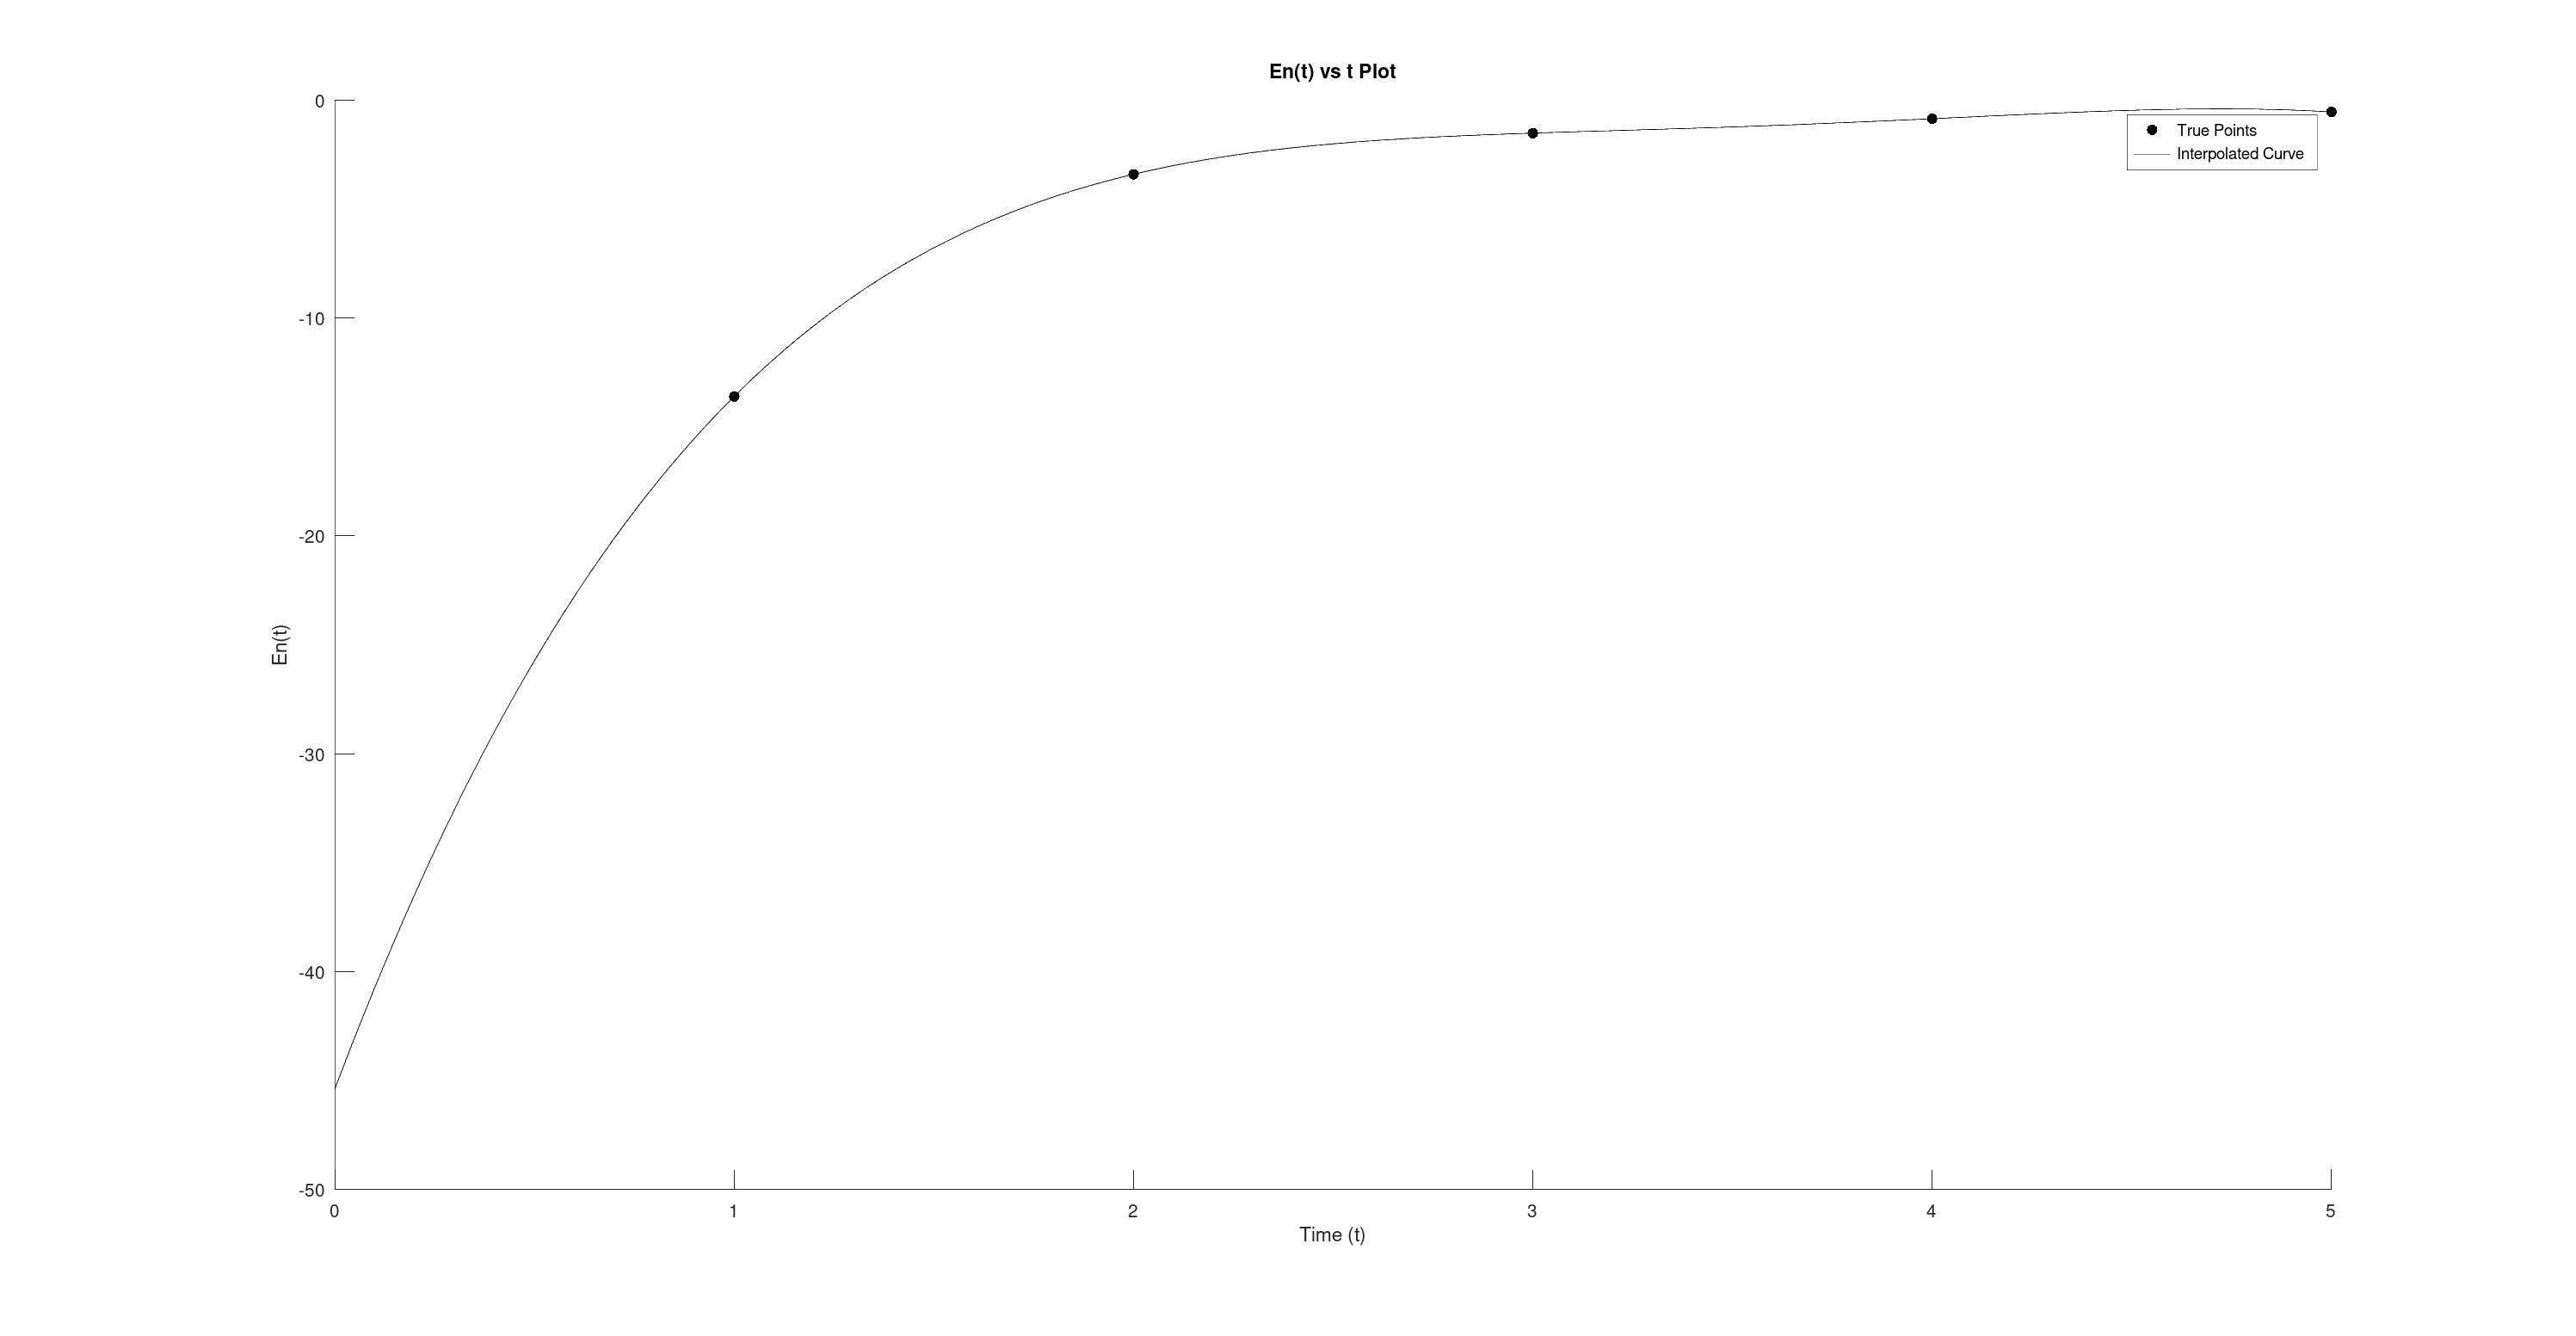
\includegraphics[width=0.9\textwidth]{a2.jpg}
  \caption{Interpolated polynomial for hydrogen atom energy levels. Discrete points (black) and interpolated curve (black line).}
\end{figure}

\section*{Conclusion}
Newton’s divided difference interpolation accurately reconstructed the energy spectrum of hydrogen from discrete quantum numbers. While the analytical formula $E_n = -13.6/n^2$ is known, this exercise illustrates how polynomial interpolation can approximate physical laws from limited data. However, interpolation beyond the given range (extrapolation) may diverge significantly, highlighting the importance of using analytical models where available.
